\documentclass[10pt,a4paper]{article}
\usepackage[utf8x]{inputenc}
\usepackage{ucs}
\usepackage[spanish]{babel}
\usepackage{amsmath}
\usepackage{amsfonts}
\usepackage{amssymb}

\usepackage{float}
\usepackage[font=small,labelfont=bf]{caption}
\usepackage{wrapfig}

\usepackage{graphicx}

\usepackage{multicol}

\author{Cristian Escudero}
\title{Resumen SO}
\begin{document}
\maketitle
\section{Tipos de SO}
El \textbf{SO} es un \textbf{administrador} de recursos: procesos, memoria, e/s, comunicaciones, usuarios, seguridad.

\subsection{Clasificación según su estructura}
\paragraph{Monolíticos.} Están constituídos por un conjunto de rutinas fuertemente entrelazadas. Aunque \textbf{eficientes}, son difíciles de modificar debido a su falta de flexibilidad.

\paragraph{Jerárquicos.} Proponen niveles de construcción del SO, que van desde el \textit{usuario} (en el más alto nivel), al \textit{hardware} (en el más bajo nivel):

\begin{quote}
\textbf{usuarios} $\rightarrow$ archivos $\rightarrow$ e/s $\rightarrow$ comunicaciones $\rightarrow$ memoria $\rightarrow$ $\mu P$ $\rightarrow$ \textbf{hardware}.
\end{quote}

El más conocido es el modelo \textbf{THE} (de Dijkstra). Otra ejemplificación jerárquica es la de \textit{anillos}, similar al THE. Los algoritmos del sistema se construyen distribuídos en cuatro anillos: del 0 (para el SO) al 3 (para las aplicaciones).

\paragraph{Cliente-Servidor.} Es el modelo más reciente. Las aplicaciones del SO pueden solicitar (\textbf{cliente}) u ofrecer (\textbf{servidor}) un procedimiento. Las aplicación puede entonces variar en cualquier momento entre ser \textit{servidor} o \textit{cliente}. El \textbf{núcleo} del sistema es el encargado de establecer todas las comunicaciones y pedidos

\paragraph{Máquina Virtual.} Se da en sistemas multiprocesos, en el cual se le  \textit{"hace creer"} al proceso que dispone de la totalidad del HW y del SO.

\subsection{Según sus servicios}
\begin{multicols}{2} 
\begin{itemize}
\item Por el nro. de usuarios:
\begin{itemize}
\item Monousuario
\item Multiusuario
\end{itemize}

\item Por el nro. de tareas:
\begin{itemize}
\item Monotarea
\item Multitarea
\end{itemize}

\item Por el nro. de procesos:
\begin{itemize}
\item Monoprocesador
\item Multiprocesador
\subitem - Asimétrico
\subitem - Simétrico
\end{itemize}
\end{itemize}
\end{multicols} 

\section{Procesos}
\subsection{Administración de Procesos}
Un \textbf{proceso} es un programa en ejecución con un entorno asociado. Está constituído por áreas de código y de datos. Esta última se divide en el área que usa efectivamente el proceso y el área de la pila.

Los SO actuales trabajan con múltiples procesos usando una técnica que se conoce como \textit{time-sharing}, que distribuye el tiempo del $\mu P$.

El tiempo asignado para uso del $\mu P$ se conoce como \textit{quantum}, y la forma en la cual el sistema conoce el tiempo que va a pasando es a través de una interrupción externa: la \textbf{IRQ0} del reloj.

Al ser la IRQ0 esencial para el manejo de la multiprogramación, los programas no pueden enmascarar interrupciones. La instrucción para enmascarar, DI, es una instrucción propia del \textit{modo protegido}.

\subsection{Cambio de Contexto y PCB}
Se produce un \textbf{cambio de contexto} cuando se pasa el control del procesador de un proceso a otro.

El \textbf{contexto} hace referencia al proceso y se expresa prácticamente en una estructura de almacenamiento conocida como \textbf{PCB} (bloque de control de proceso). El SO genera un PCB para cada proceso que se crea.

\begin{wrapfigure}{r}{0.3\textwidth}
  \label{fig1}
  \centering
  \hbox{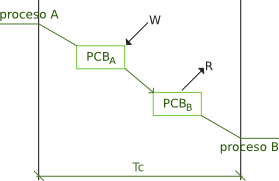
\includegraphics[width=0.6\textwidth-\fboxrule-\fboxrule]{fig1.png}}  
\end{wrapfigure}

La conmutación entre un proceso y otro exige la actualización del PCB del proceso que se deja y la lectura del PCB del proceso que va a tomar al $\mu P$. Esta acción de cambio de contexto debe durar el \textbf{menor tiempo posible}, ya que es uno los indicadores del uso del procesador:
\[E= \frac{T_p}{T_c+T_p} \cdot 100 \% \]

Normalmente el PCB contiene la siguiente información:
\begin{itemize}
\item Archivos/recursos en uso.
\item Contenido de los registros internos del procesador.
\item Ocupación de memoria externa/interna.
\item Privilegios.
\end{itemize}

\subsection{Estados de Proceso}
Se pueden dividir en \textbf{activos} e \textbf{inactivos}.
Entre los activos encontramos los estados de \textbf{ejecución}, \textbf{preparado} y \textbf{bloqueado}.

Los dos primeros están relacionados con el uso del procesador y es fácil reconocerlos en el \textit{time-sharing}. Un proceso está \textit{bloqueado} cuando en su ejecución se solicita un recurso que no está disponible.

Entre los estados inactivos encontramos los estados de \textbf{suspendidos} divididos en \textbf{bloqueados} y \textbf{preparados}.

\begin{figure}[h!]
  \label{fig12}
  \centering
  \hbox{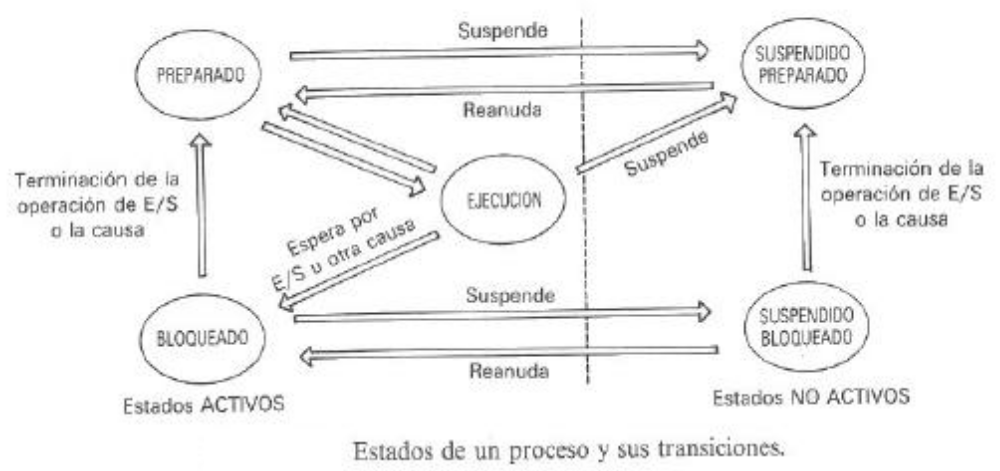
\includegraphics[width=\textwidth-\fboxrule-\fboxrule]{fig2.png}}  
\end{figure}

\subsection{Operaciones sobre Procesos}
La creación de procesos en cualquier sistema se realiza normalmente a partir de cuatro métodos:
\begin{enumerate}
\item Desde la \textbf{inicialización} sea porque se encuentra en el listado del sistema o en alguno de los registros de inicialización/configuración.
\item Porque lo ejecuta otro proceso.
\item Porque lo ejecuta el usuario, a través del \textit{shell}.
\item Porque está incluído en un archivo por lotes.
\end{enumerate}

La creación de los procesos puede ser \textbf{jerárquica} o \textbf{no jerárquica}. En el primero el hijo hereda parte del entorno del proceso padre, y si se elimina el proceso padre, al mismo tiempo se eliminan todos sus procesos hijos. En una creación \textit{no jerárquica}, el proceso es independiente de su creador.

Todas las operaciones o acciones sobre los procesos se realizan o ejecutan a partir de llamadas al SO. Será un \textbf{fork} (unix/linux) o un \textbf{createprocess} (windows/api) para crear un proceso, un \textbf{kill} o \textbf{terminateprocess} para eliminarlo, o un \textbf{exit} o \textbf{exitprocess} para terminarlo.

\subsection{Modificación de Privilegios}
Los privilegios de un proceso pueden ser:
\begin{itemize}
\item \textbf{Estáticos.} No cambian durante toda la "\textit{vida}" del proceso.
\item \textbf{Dinámicos.} Pueden ser modificados a través del usuario o del SO.
\end{itemize}
Lo normal de los sistemas actuales es que el SO modifique los privilegios entre diferentes niveles. Un proceso normalmente se inicia con un nivel en particular y su valor se modifica por más o menos a partir de este.

\subsection{Subprocesos}
Son hijos de otro proceso, que heredan el entorno de éste pero que no lo necesitan cuando se ejecutan los cambios de contexto. De esta forma, la única diferencia entre "\textit{hermanos}" es sólo el contenido de los registros internos del $\mu P$. 

Para la administración de subprocesos el SO maneja una tabla de subprocesos.

\subsection{Tipos de Procesos}
\begin{itemize}
\item \textbf{Según su código.}
\subitem \textbf{- Reutilizables.} Tienen datos asociados de manera que si vuelven a ejecutarse deben comenzar en su estado inicial.
\subitem \textbf{- Reentrantes.} No tienen datos asociados, son "\textit{puro código}".

\item \textbf{Según su acceso al procesador.}
\subitem \textbf{- Apropiativos.} Hacen uso del $\mu P$ y no lo liberan hasta que terminan.
\subitem \textbf{- No apropiativos}. Ceden en algún momento el uso del $\mu P$ antes de terminar efectivamente.

\item \textbf{Según su forma de ejecución.}
\subitem \textbf{- Residentes.} Permanecen en la memoria durante toda su ejecución.
\subitem \textbf{- Intercambiables.} Podrán ser llevados al área de \textit{intercambio} en el disco.
\end{itemize}

\subsection{Planificación de Procesos}
Sus objetivos son: justicia, máxima capacidad de ejecución, máximo número de usuarios, predecibilidad, minimización de la carga, equilibrio en el uso de recursos, y seguridad en las prioridades.

\subsubsection{Planificación a Corto Plazo}
Los procesos pueden ser:
\begin{itemize}
\item \textbf{De políticas apropiativas.} Temporalmente suspenden la ejecución de un proceso para ejecutar otro.
\item \textbf{De políticas no apropiativas.} Dejan que un proceso haga uso del $\mu P$ ahsta que dicho proceso termine.
\end{itemize}
\end{document}